\chapter{Planning}
\label{chap:planning}

The planning will be done in two parts.
The first one will follow a sequential model until the blocking points are done.
The second one will be a methodology by iteration to complete the milestone about the application interface and the next.
The method will change because the number of features isn't known yet and the needs can change.

The following figure \ref{fig:planning1} shows the different steps of the project and how the milestone will be achieved.

\begin{figure}[ht]
    \centering
    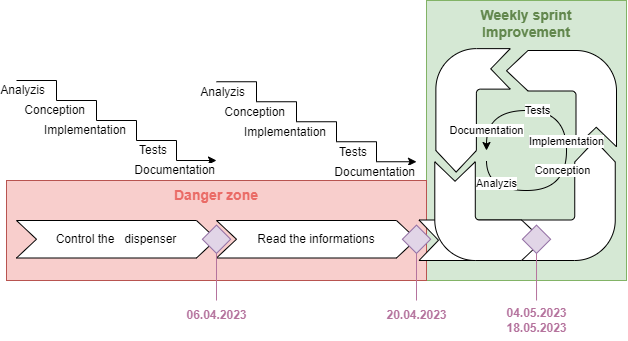
\includegraphics[width=1\textwidth]{img/planning.drawio.png}
    \caption{Planning}
    \label{fig:planning1}
\end{figure}

\section{Danger zone}
\label{sec:planning:danger}

The danger zone is the part of the project where the blocking points are.
It represents by the red part of the figure \ref{fig:planning} these steps are required to go further in the project.
This part will be managed with \href{https://gitlab.forge.hefr.ch/ps6-2223-microdoser/ps6-2223-microdoser/-/milestones/3#tab-issues}{the milestones view of Gitlab}.

\section{Iterations}
\label{sec:planning:iterations}

The agile part will be done with \href{https://gitlab.forge.hefr.ch/ps6-2223-microdoser/ps6-2223-microdoser/-/cadences}{the iterations view of Gitlab}.
The iterations will be done every week and the project will be improved during this time.
For now, just the two first milestones are planned and every week's tasks will be displayed on this \href{https://gitlab.forge.hefr.ch/ps6-2223-microdoser/ps6-2223-microdoser/-/boards/1667?iteration_id=Current}{board}.


\section{Milestones}
\label{sec:planning:milestones}

The milestones are the mandatory goals of the project.
A milestone has been added at the end of the project to improve it by adding or optimizing features.
The milestones can be easily found at this \href{https://gitlab.forge.hefr.ch/ps6-2223-microdoser/ps6-2223-microdoser/-/milestones}{link}.

\section{Issues}
\label{sec:planning:issues}

The issues are representing the tasks that need to be done to complete a milestone.
They can be detailed with a checklist to specify the steps to follow and they can be linked to a merge request to keep a reference to the code that solves the issue.
The weight of an issue is used to estimate the time needed to complete it and one weight unit is equivalent to two hours of work.
The list of issues can be found on this \href{https://gitlab.forge.hefr.ch/ps6-2223-microdoser/ps6-2223-microdoser/-/boards/1658}{board}.

